\documentclass{article}
\usepackage{pdflscape}
\usepackage[margin=1in]{geometry}
\usepackage{verbatim}
\usepackage{graphicx, float}
\author{Astrid Augusta Yu}
\title{CPE 233 Lab \#3 -- Arithmetic Logic Unit}
\date{\today}

\usepackage{amsmath}
\usepackage{amsfonts}
\usepackage{amssymb}
\DeclareMathOperator\bit{bit}
\DeclareMathOperator\byte{byte}
\DeclareMathOperator\word{word}

\begin{document}
\maketitle

\section{Questions}

\begin{enumerate}
    \item \textbf{Briefly describe what (or who) determines the number 
    of instruction formats a given instruction set contains. }
    
    The people who designed the instruction set determine how many instruction formats 
    there are. 

    \item \textbf{List the six RISC-V MCU instruction formats. }
    
    R, I, S, B, U, J
    \item \textbf{The design of the RISC-V MCU ISA intentionally shares as many fields as possible in the six
    different instruction formats. Briefly explain the reason why the ISA designers did this.  }
    
    The designers did this in order to reduce the amount of hardware 
        needed to decode and execute the instructions. By sharing fields,
        you can use the same hardware to decode different instructions.
    \item \textbf{In the RISC-V MCU ISA, a given bit location in one instruction does one thing for one
    instruction and something else for another instruction. This means that bit is connected to the
    inputs on two different devices. Briefly explain why this sharing of signals not a problem.
     You can typically use assembly language to make a given program written in a higher-level }
    
    This is not a problem because the signal types are differentiated
        using opcodes. Opcodes designate what the instructions should be
        treated as.
    \item \textbf{You can typically use assembly language to make a given program written in a higher-level
    language run faster. Briefly but fully explain this concept.  }
    
    Higher-level languages often run slower because, although the 
        compilers are getting better at optimizing, humans can often make even 
        better optimizations by writing the assembly directly.
    \item \textbf{We refer to computer languages such as C and Java as being “portable”. Define this term in your
    own words.  }
    
    C and Java being portable means that the same code can run on many different systems and architectures with 
    little to no changes required, so long as there is a working compiler that targets that system.
    \item \textbf{Assembly languages, on the other hand, are not portable. Briefly describe why assembly
    languages are not portable.  }
    
    Assembly is not portable because different processor architectures 
        have completely different instruction sets.
    \item \textbf{Program control instructions rely on labels in the code to be encoded and subsequently work
    properly. If you look at the machine code for a program, it contains no labels. Briefly explain how
    does the machine code get away with not encoding labels?  }
    
    The assembler converts the labels into addresses, and at each 
        usage of the label, the address is converted into a relative address.
    \item \textbf{Is it possible to have two of the same labels in an assembly language program? Briefly but
    completely explain.  } 
    
    No. It wouldn't make sense because the assembler can't tell which
        address to resolve the reference to. 
    \item \textbf{Is it possible to have two or more labels in an assembly language program with the same
    numerical value? Briefly but completely explain.  } 

    Yes. In that case, they would both point to the same address. 
    \item \textbf{Can you write a RISC-V MCU assembly language program that “stops running”? Briefly explain
    your answer.  }
    
    Having a jump that jumps to itself effectively makes the program stop running. However, 
    will waste power while doing so unless the MCU has a low-power mode feature that the .
    code can enable.
    \item \textbf{Briefly describe at least two limitations of the RISC-V OTTER ALU. }
    
    The ALU cannot multiply or divide by arbitrary integers. This would
        have to be implemented by additional hardware or by code implementing
        multiplication/division. Additionally, it cannot process floating-point 
        numbers. There needs to be a FPU in order for that to happen without any 
        extra software.
\end{enumerate}

\section{Programming Assignment}

\begin{verbatim}
;----------------------------------------------------------------
;- Sums 10 unsigned word values from the input port addressed by 
;- 0xC000_CCCC and returns the upper 16 bits of the sum.
;-
;- Tweaked registers: t0, t1, t2, x30
;----------------------------------------------------------------
init:
    li t0, 0xC000CCCC       # t0 = the input port
    li t1, 10               # t1 = times to read left
    li x30, 0               # x30 = accumulator

load:
    lw t2, t0               # t2 = value from I/O
    add x30, x30, t2        # x30 += t2
    addi t1, t1, -1         # decrement counter
    bgt t1, zero, load      # repeat while t0 has not reached end

    li t1, 0xFFFF           # t1 = maximum allowable number
    ble x30, t1, done       # end early if x30 <= t1
divide:
    srli x30, x30, 1        # divide x30 by 2
    bgt x30, t1, divide     # repeat while x30 > t1

done:
    ret
\end{verbatim}

\section{Hardware Design Assignment}

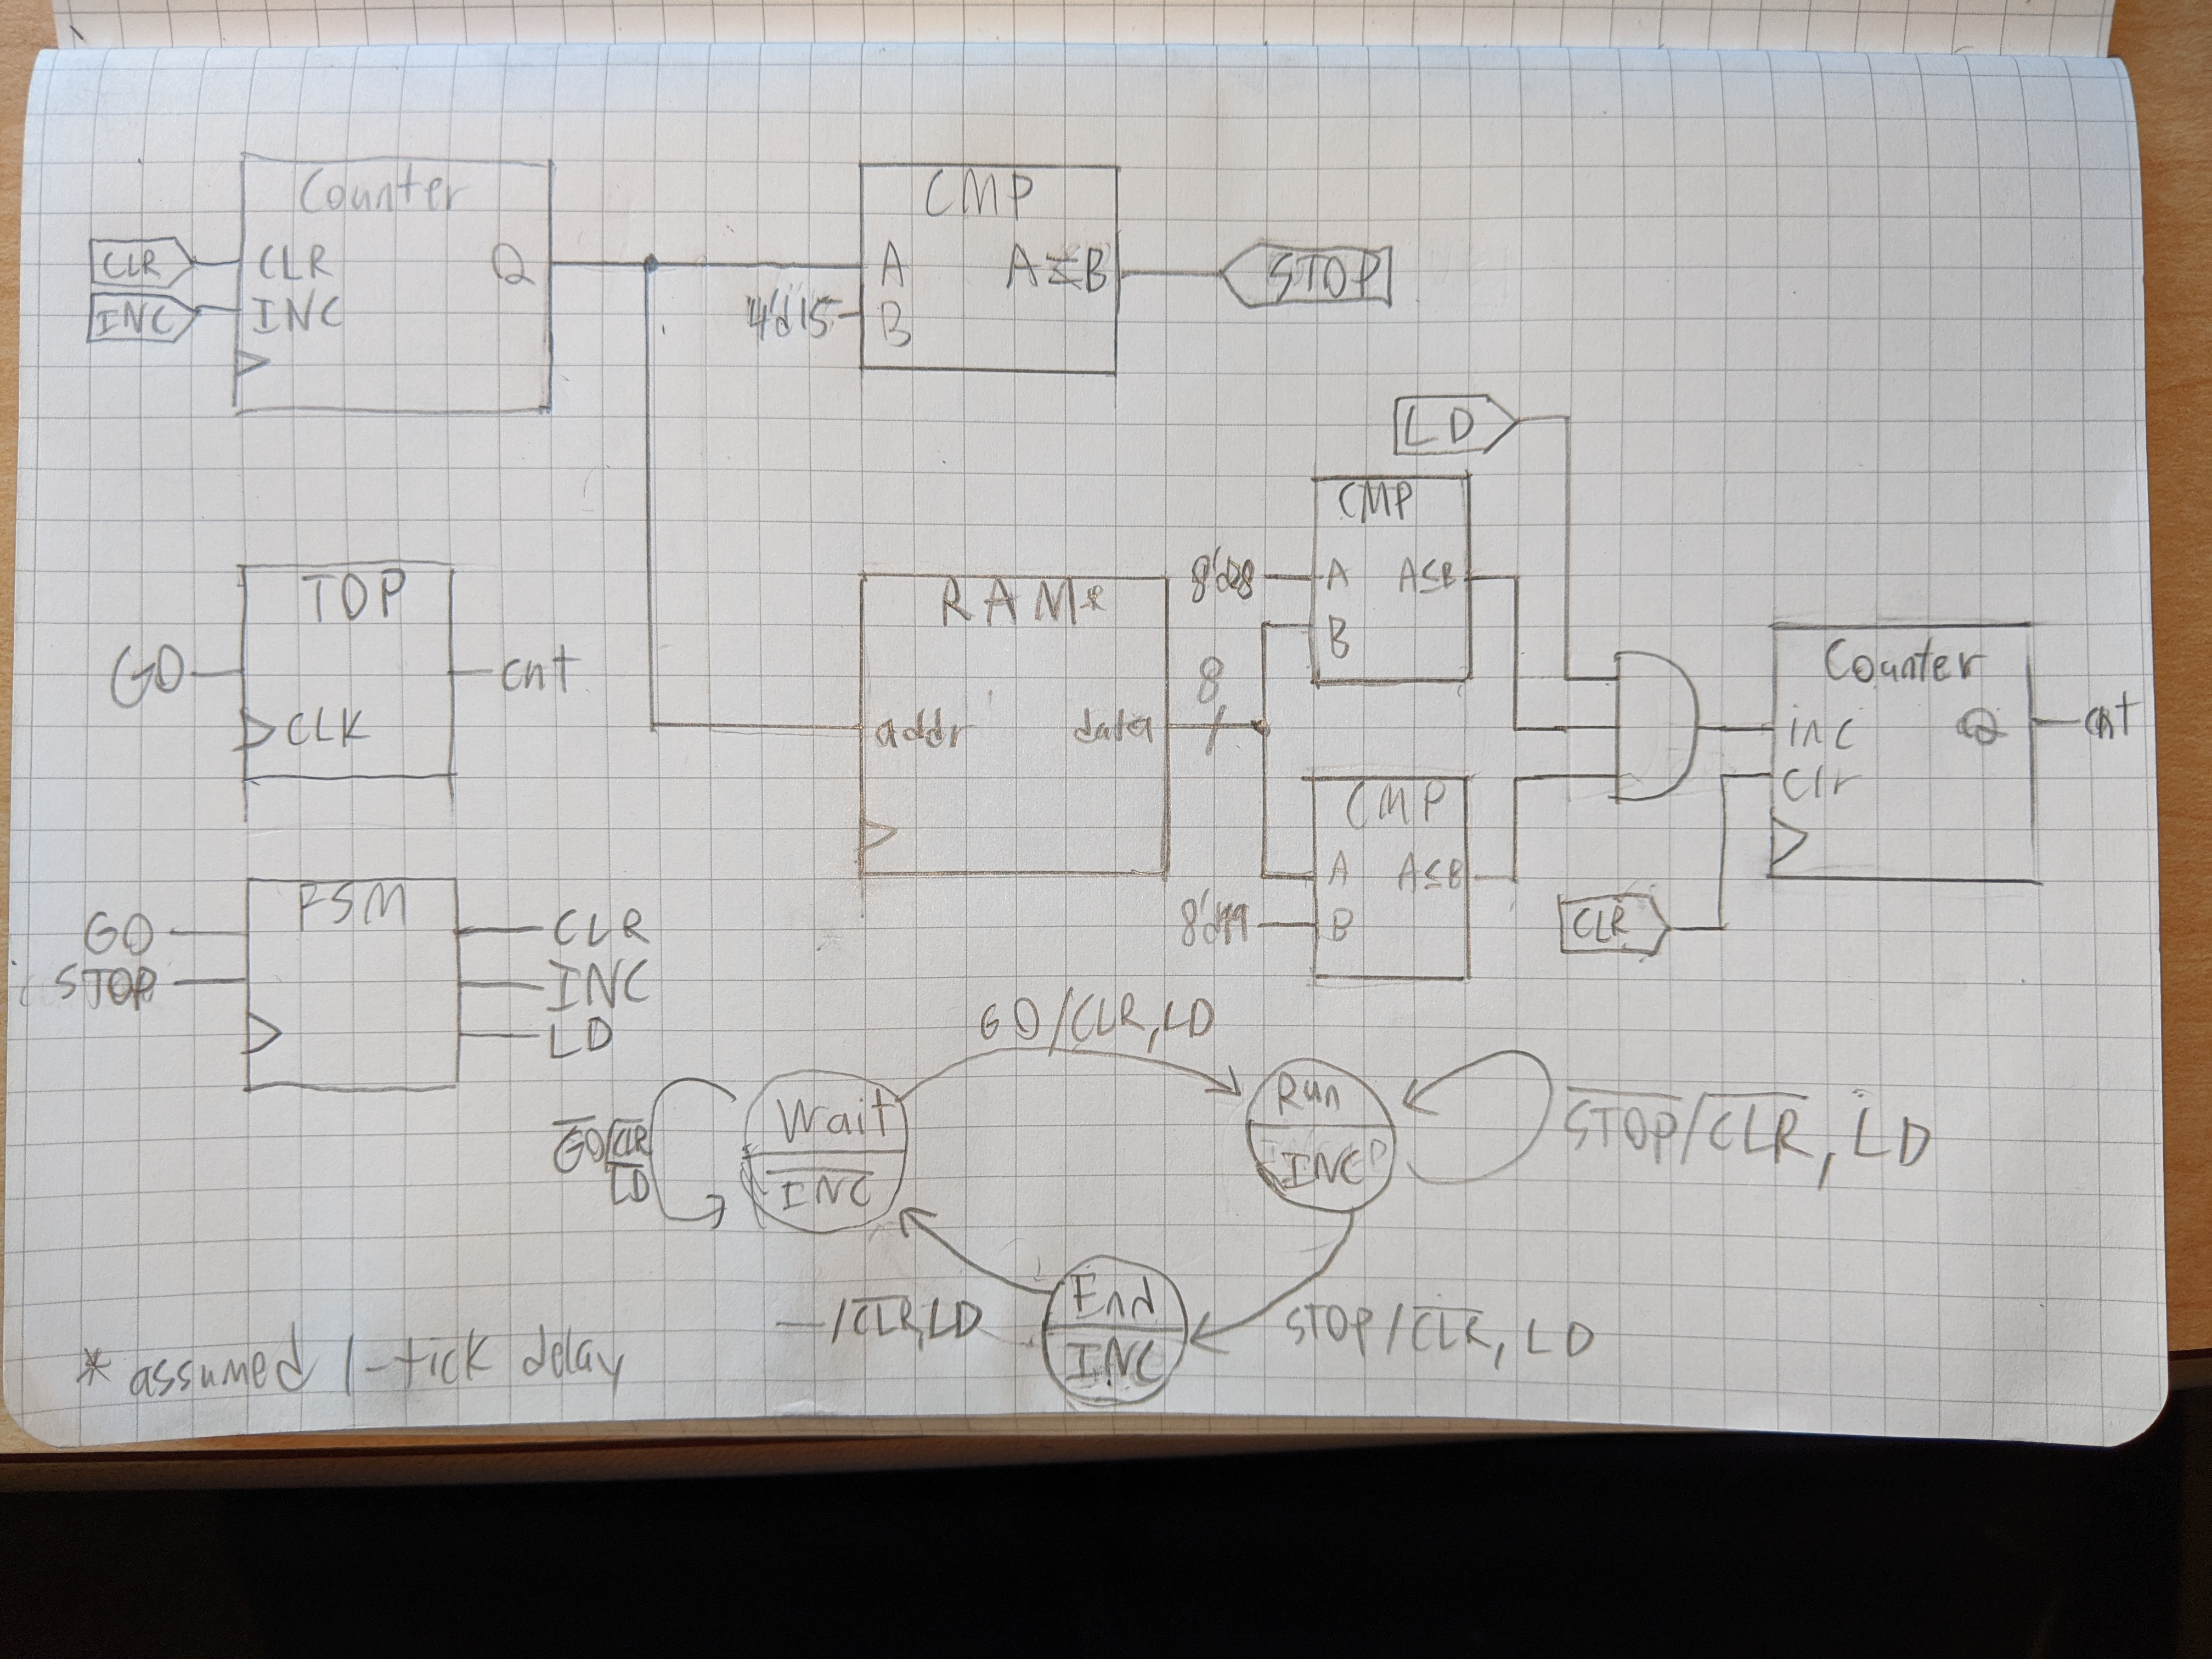
\includegraphics[width=\linewidth]{hw.jpg}

\section{HDL}

\subsection{alu.sv}
\begin{verbatim}
`timescale 1ns / 1ps
//////////////////////////////////////////////////////////////////////////////////
// Company: Cal Poly
// Engineer: Astrid Yu
// 
// Create Date: 04/19/2020 08:07:54 PM
// Design Name: Otter MCU ALU
// Module Name: alu
// Project Name: 
// Target Devices: 
// Tool Versions: 
// Description: Performs arithmetic operations for the Otter MCU.
// 
// Dependencies: 
// 
// Revision:
// Revision 0.01 - File Created
// Additional Comments:
// 
//////////////////////////////////////////////////////////////////////////////////


module alu(
    input [31:0] srcA,
    input [31:0] srcB,
    input [3:0] alu_fun,
    output logic [31:0] result
    );
        
    always_comb begin
        case (alu_fun)
            4'b0000: result = srcA + srcB;                      // add
            4'b1000: result = srcA - srcB;                      // sub
            4'b0110: result = srcA | srcB;                      // or
            4'b0111: result = srcA & srcB;                      // and
            4'b0100: result = srcA ^ srcB;                      // xor 
            4'b0101: result = srcA >> srcB;                     // srl
            4'b0001: result = srcA << srcB;                     // sll
            4'b1101: result = srcA >>> srcB;                    // sra
            4'b0010: result = $signed(srcA) < $signed(srcB);    // slt
            4'b0011: result = srcA < srcB;                      // sltu
            4'b1001: result = srcA;                             // lui
            default: result = 32'hDEADBEEF;
        endcase
    end
endmodule

\end{verbatim}

\begin{landscape}
\section{Timing Diagram}

\subsection{Waveform Output}
\includegraphics[width=\linewidth]{w.png}

\subsection{Table Summary}

\begin{center}
\begin{tabular}{| c | c | c | c | c |}

    \hline
    \texttt{alu\_fun} & Instruction & \texttt{srcA} & \texttt{srcB} & \texttt{result} \\
    \hline
    0000 & add  & 25 & 26 & 51 \\ 
    1000 & sub  & 25 & 26 & -1 \\ 
    1000 & sub  & -1 & 1 & -2 \\ 
    0110 & or   & 0xaaaa & 0x5555 & 0xffff \\ 
    0111 & and  & 0xaaaa & 0x5555 & 0x0000 \\ 
    0100 & xor  & 0xaaaa & 0x5555 & 0xffff \\ 
    0101 & srl  & 0xff00 & 5 & 0x000007f8 \\ 
    0001 & sll  & 0xff00 & 5 & 0x001fe000 \\ 
    1101 & sra  & 0x8000ff00 & 5 & 0x40007f8 \\ 
    0010 & slt  & 2147548928 & 5 & 1 \\ 
    0011 & sltu & 2147548928 & 5 & 0 \\ 
    1001 & lui  & 0x0000ff00 & 0x0fff & 0x0000ff00 \\ 
    0011 & sltu & 2147548928 & 0x0fff & 0 \\ 
    1100 & (invalid) & 0x8000ff00 & 0x0fff & 0xdeadbeef \\ 
    \hline

\end{tabular}
\end{center}

\end{landscape}

    
\end{document}